\documentclass[a4paper, 14pt]{extarticle}

% Поля
%--------------------------------------
\usepackage{geometry}
\geometry{a4paper,tmargin=2cm,bmargin=2cm,lmargin=3cm,rmargin=1cm}
%--------------------------------------


%Russian-specific packages
%--------------------------------------
\usepackage[T2A]{fontenc}
\usepackage[utf8]{inputenc} 
\usepackage[english, main=russian]{babel}
%--------------------------------------

\usepackage{textcomp}

% Красная строка
%--------------------------------------
\usepackage{indentfirst}               
%--------------------------------------             


%Graphics
%--------------------------------------
\usepackage{graphicx}
\graphicspath{ {./images/} }
\usepackage{wrapfig}
%--------------------------------------

% Полуторный интервал
%--------------------------------------
\linespread{1.3}                    
%--------------------------------------

%Выравнивание и переносы
%--------------------------------------
% Избавляемся от переполнений
\sloppy
% Запрещаем разрыв страницы после первой строки абзаца
\clubpenalty=10000
% Запрещаем разрыв страницы после последней строки абзаца
\widowpenalty=10000
%--------------------------------------

%Списки
\usepackage{enumitem}

%Подписи
\usepackage{caption} 

%Гиперссылки
\usepackage{hyperref}

\hypersetup {
	unicode=true
}

%Рисунки
%--------------------------------------
\DeclareCaptionLabelSeparator*{emdash}{~--- }
\captionsetup[figure]{labelsep=emdash,font=onehalfspacing,position=bottom}
%--------------------------------------

\usepackage{tempora}

%Листинги
%--------------------------------------
\usepackage{listings}
\lstset{
  basicstyle=\ttfamily\footnotesize, 
  %basicstyle=\footnotesize\AnkaCoder,        % the size of the fonts that are used for the code
  breakatwhitespace=false,         % sets if automatic breaks shoulbd only happen at whitespace
  breaklines=true,                 % sets automatic line breaking
  captionpos=t,                    % sets the caption-position to bottom
  inputencoding=utf8,
  frame=single,                    % adds a frame around the code
  keepspaces=true,                 % keeps spaces in text, useful for keeping indentation of code (possibly needs columns=flexible)
  keywordstyle=\bf,       % keyword style
  numbers=left,                    % where to put the line-numbers; possible values are (none, left, right)
  numbersep=5pt,                   % how far the line-numbers are from the code
  xleftmargin=25pt,
  xrightmargin=25pt,
  showspaces=false,                % show spaces everywhere adding particular underscores; it overrides 'showstringspaces'
  showstringspaces=false,          % underline spaces within strings only
  showtabs=false,                  % show tabs within strings adding particular underscores
  stepnumber=1,                    % the step between two line-numbers. If it's 1, each line will be numbered
  tabsize=2,                       % sets default tabsize to 8 spaces
  title=\lstname                   % show the filename of files included with \lstinputlisting; also try caption instead of title
}
%--------------------------------------

%%% Математические пакеты %%%
%--------------------------------------
\usepackage{amsthm,amsfonts,amsmath,amssymb,amscd}  % Математические дополнения от AMS
\usepackage{mathtools}                              % Добавляет окружение multlined
\usepackage[perpage]{footmisc}
%--------------------------------------

%--------------------------------------
%			НАЧАЛО ДОКУМЕНТА
%--------------------------------------

\begin{document}

%--------------------------------------
%			ТИТУЛЬНЫЙ ЛИСТ
%--------------------------------------
\begin{titlepage}
\thispagestyle{empty}
\newpage


%Шапка титульного листа
%--------------------------------------
\vspace*{-60pt}
\hspace{-65pt}
\begin{minipage}{0.3\textwidth}
\hspace*{-20pt}\centering

\includegraphics[width=\textwidth]{emblem}
\end{minipage}
\begin{minipage}{0.67\textwidth}\small \textbf{
\vspace*{-0.7ex}
\hspace*{-6pt}\centerline{Министерство науки и высшего образования Российской Федерации}
\vspace*{-0.7ex}
\centerline{Федеральное государственное бюджетное образовательное учреждение }
\vspace*{-0.7ex}
\centerline{высшего образования}
\vspace*{-0.7ex}
\centerline{<<Московский государственный технический университет}
\vspace*{-0.7ex}
\centerline{имени Н.Э. Баумана}
\vspace*{-0.7ex}
\centerline{(национальный исследовательский университет)>>}
\vspace*{-0.7ex}
\centerline{(МГТУ им. Н.Э. Баумана)}}
\end{minipage}
%--------------------------------------

%Полосы
%--------------------------------------
\vspace{-25pt}
\hspace{-35pt}\rule{\textwidth}{2.3pt}

\vspace*{-20.3pt}
\hspace{-35pt}\rule{\textwidth}{0.4pt}
%--------------------------------------

\vspace{1.5ex}
\hspace{-35pt} \noindent \small ФАКУЛЬТЕТ\hspace{80pt} <<Информатика и системы управления>>

\vspace*{-16pt}
\hspace{47pt}\rule{0.83\textwidth}{0.4pt}

\vspace{0.5ex}
\hspace{-35pt} \noindent \small КАФЕДРА\hspace{50pt} <<Теоретическая информатика и компьютерные технологии>>

\vspace*{-16pt}
\hspace{30pt}\rule{0.866\textwidth}{0.4pt}
  
\vspace{11em}

\begin{center}
\Large {\bf Лабораторная работа № 12} \\ 
\large {\bf по курсу <<Языки и методы программирования>>} \\
\large <<Обработка текстовых файлов>> 
\end{center}\normalsize

\vspace{8em}


\begin{flushright}
  {Студент группы ИУ9-21Б Горбунов А. Д. \hspace*{15pt}\\ 
  \vspace{2ex}
  Преподаватель Посевин Д. П.\hspace*{15pt}}
\end{flushright}

\bigskip

\vfill
 

\begin{center}
\textsl{Москва 2023}
\end{center}
\end{titlepage}
%--------------------------------------
%		КОНЕЦ ТИТУЛЬНОГО ЛИСТА
%--------------------------------------

\renewcommand{\ttdefault}{pcr}

\setlength{\tabcolsep}{3pt}
\newpage
\setcounter{page}{2}

\section{Задание}\label{Sect::task}
    Найти все файлы с расширением «html» в заданномкаталоге, для каждого файла очистить его текст от скриптов и сохранить в файл с тем же именем в текущий каталог. Скрипты в HTML-файле записываются внутри тега script.
    
    Например:
    
    <script>
    
        document.getElementById("demo").innerHTML = " Hello JavaScript!";
        
    </script>
    
    Работоспособность программы нужно проверить на наборе HTML-файлов, загруженных из интернета.
\section{Результаты}\label{Sect::res}

Исходный код программы представлен в листинге~\ref{lst:code1}, ~\ref{lst:code2}, ~\ref{lst:code3}

\begin{figure}[!htb]
\begin{lstlisting}[language={c++},caption={main.cpp},label={lst:code1}]
#include <iostream>
#include <cstring>
#include <sys/types.h>
#include <dirent.h>
#include <fstream>
using namespace std;
int main(int argc, char *argv[])
{
    if (argc != 2) {
        cout << "Usage: " << argv[0] << " directoryPath" << endl;
        return 1;
    }
    DIR *dir = opendir(argv[1]);
    if (dir == NULL)
    {
        cout << "Failed to open directory!" << endl;
        return 1;
    }
    struct dirent *ent;
    char path[1000], outfilename[1000], buffer[1024];
    ifstream infile;
    ofstream outfile;
\end{lstlisting}
\end{figure}

\begin{figure}[!htb]
\begin{lstlisting}[language={c++},caption={main.cpp},label={lst:code2}]
    while ((ent = readdir(dir)) != NULL)
        if (ent->d_type == DT_REG && strstr(ent->d_name, ".html"))
        {
            cout << "Processing file " << ent->d_name << "..." << endl;
            strcpy(path, argv[1]);
            strcat(path, "/");
            strcat(path, ent->d_name);
            infile.open(path);
            if (!infile.is_open())
            {
                cout << "Failed to open input file!" << endl;
                return 1;
            }
            strcpy(outfilename, ent->d_name);
            outfile.open(outfilename);
            if (!outfile.is_open())
            {
                cout << "Failed to open output file!" << endl;
                return 1;
            }
            bool in_script = false;
            while(infile.getline(buffer, 1024))
            {
                char *pos = buffer;
                while (*pos)
                {
                    if (in_script)
                        if (strncmp(pos, "</script>", 9) == 0)
                        {
                            pos += 9;
                            in_script = false;
                        }
                        else
                            ++pos;
                    else
                    {
                        char *start = strstr(pos, "<script>");
                        if (start)
                        {
                            outfile.write(pos, start-pos);
                            pos = start;
                            in_script = true;
                        }
                        else
                        {
                            outfile << *pos;
                            if(*pos++ =='>' ){
                            	outfile << endl;
                            }
                        }
                    }
                }
                if (in_script)
                {
                    outfile << endl;
                }
            }
            infile.close();
            outfile.close();
        }
    closedir(dir);
    return 0;
}
\end{lstlisting}
\end{figure}

\begin{figure}[!htb]
\begin{lstlisting}[language={html},caption={Один из html файлов},label={lst:code3}]
<!DOCTYPE html>
<html>
    <head>
        <meta charset="UTF-8">
        <title>Script example JavaScript </title>
    </head>
    <body>
        <script>
            alert("Hello, world!");
        </script>
    </body>
</html>
\end{lstlisting}
\end{figure}

\begin{figure}[!htb]
Результат запуска представлен на рисунке ~\ref{fig:picture_1.png}, ~\ref{fig:picture_2.png}, ~\ref{fig:picture_3.png}, ~\ref{fig:picture_4.png}
\end{figure}

\begin{figure}[!htb]
	\centering
	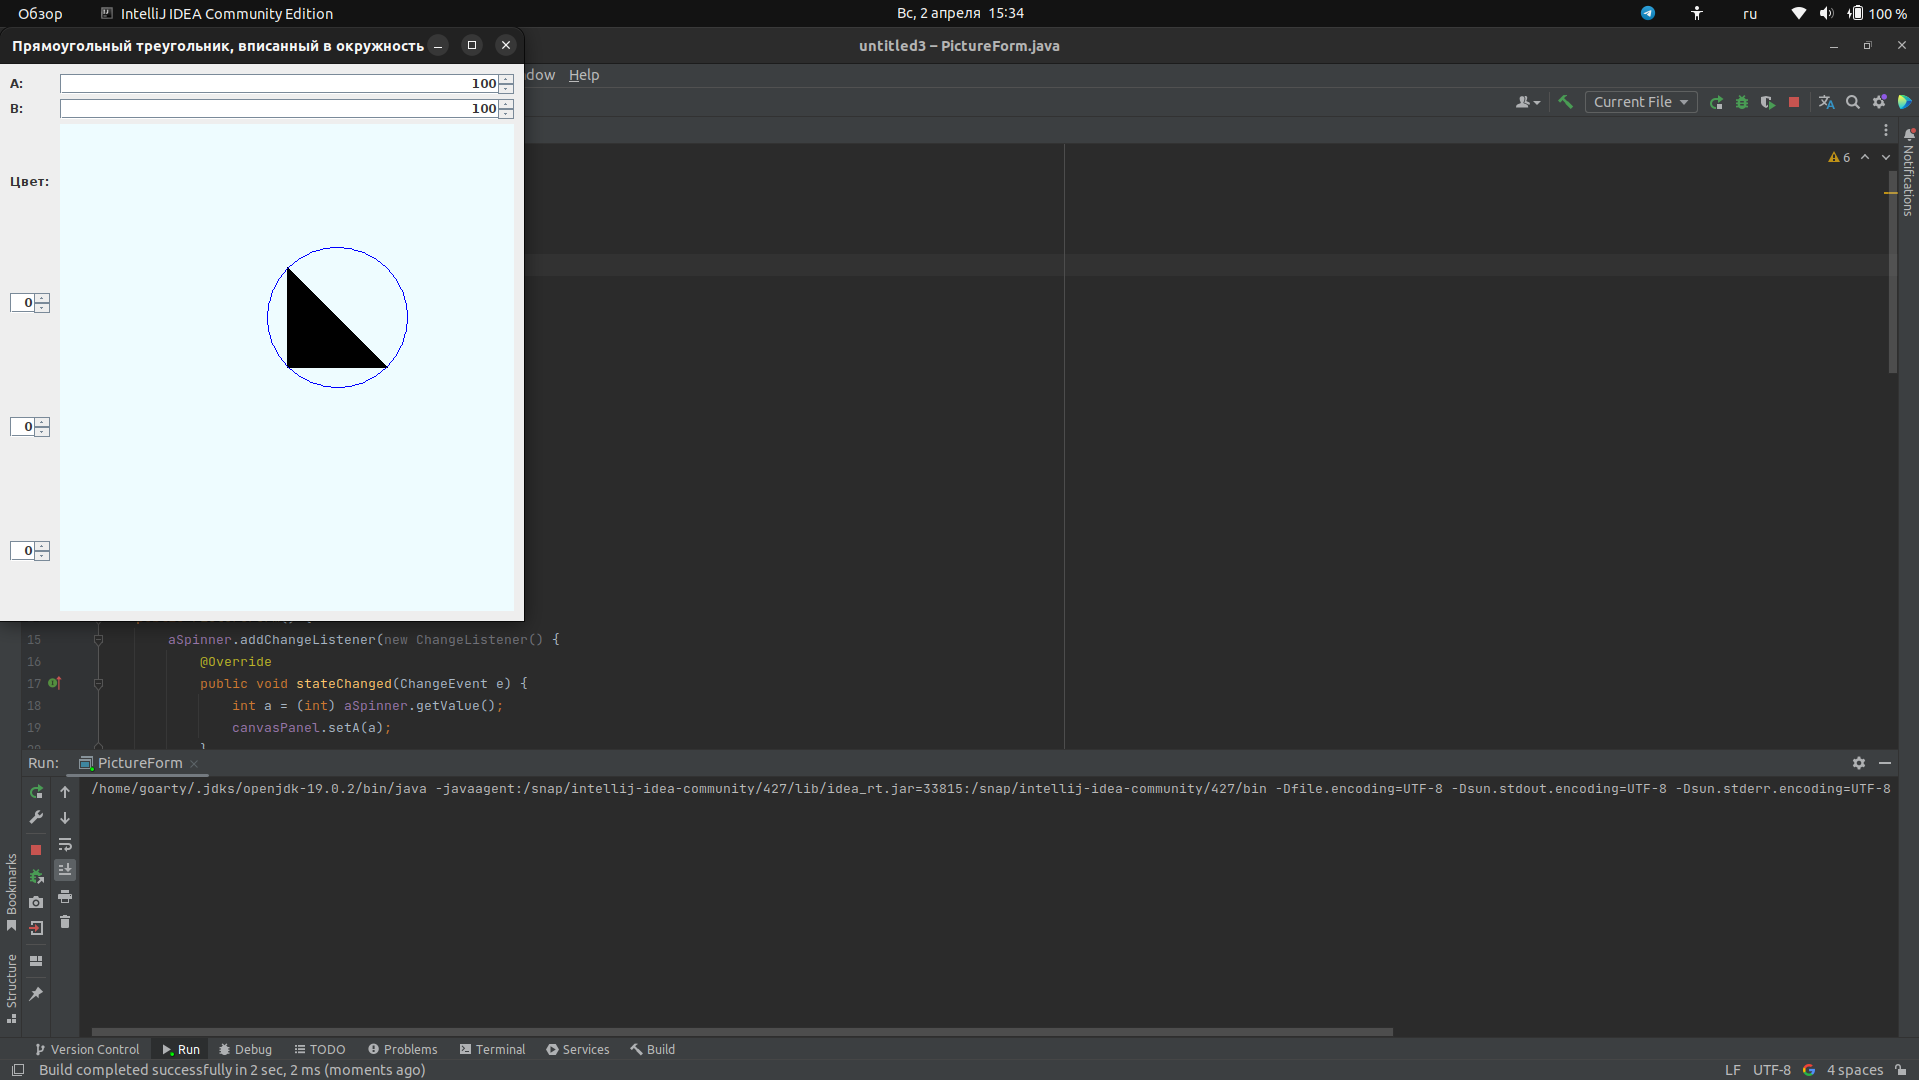
\includegraphics[width=0.8\textwidth]{picture_1.png}
\caption{Реализация main.cpp}
\label{fig:picture_1.png}
\end{figure}

\begin{figure}[!htb]
	\centering
	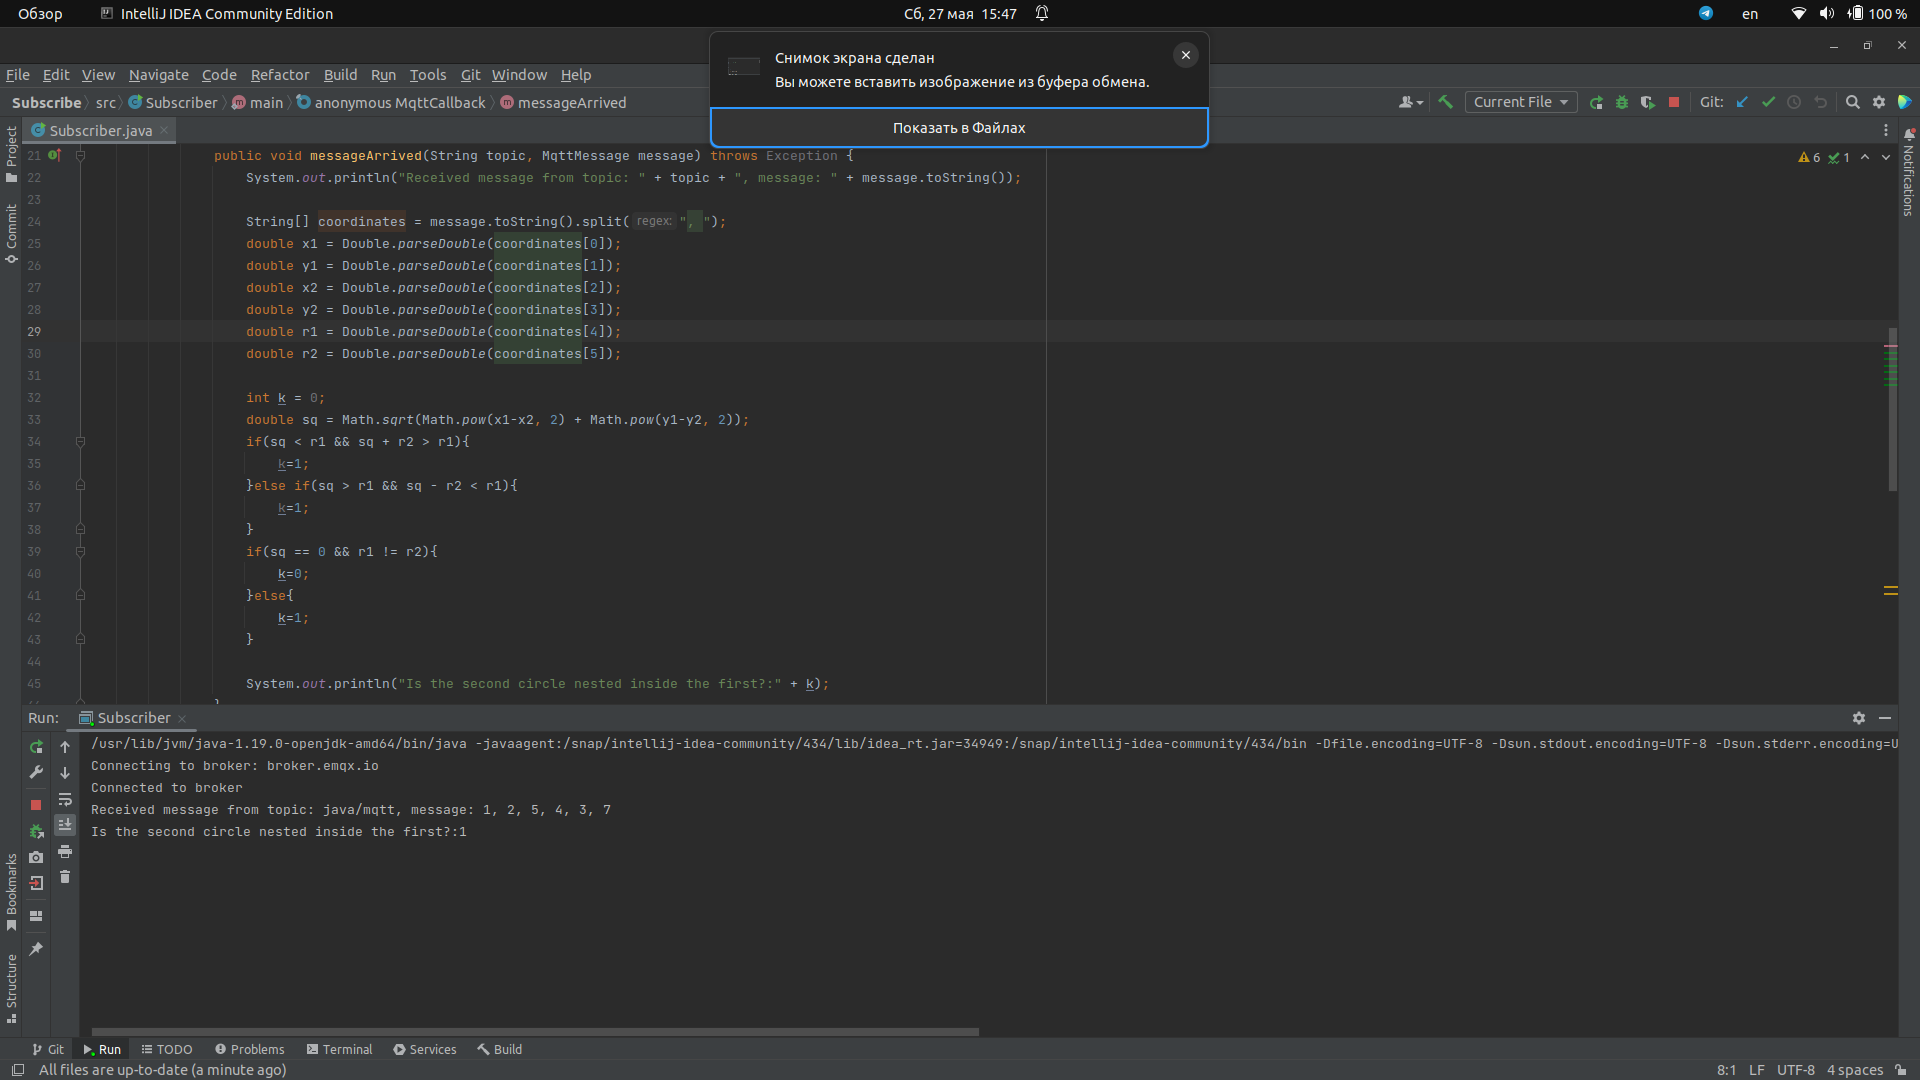
\includegraphics[width=0.8\textwidth]{picture_2.png}
\caption{Реализация main.cpp(продолжение)}
\label{fig:picture_2.png}
\end{figure}

\begin{figure}[!htb]
	\centering
	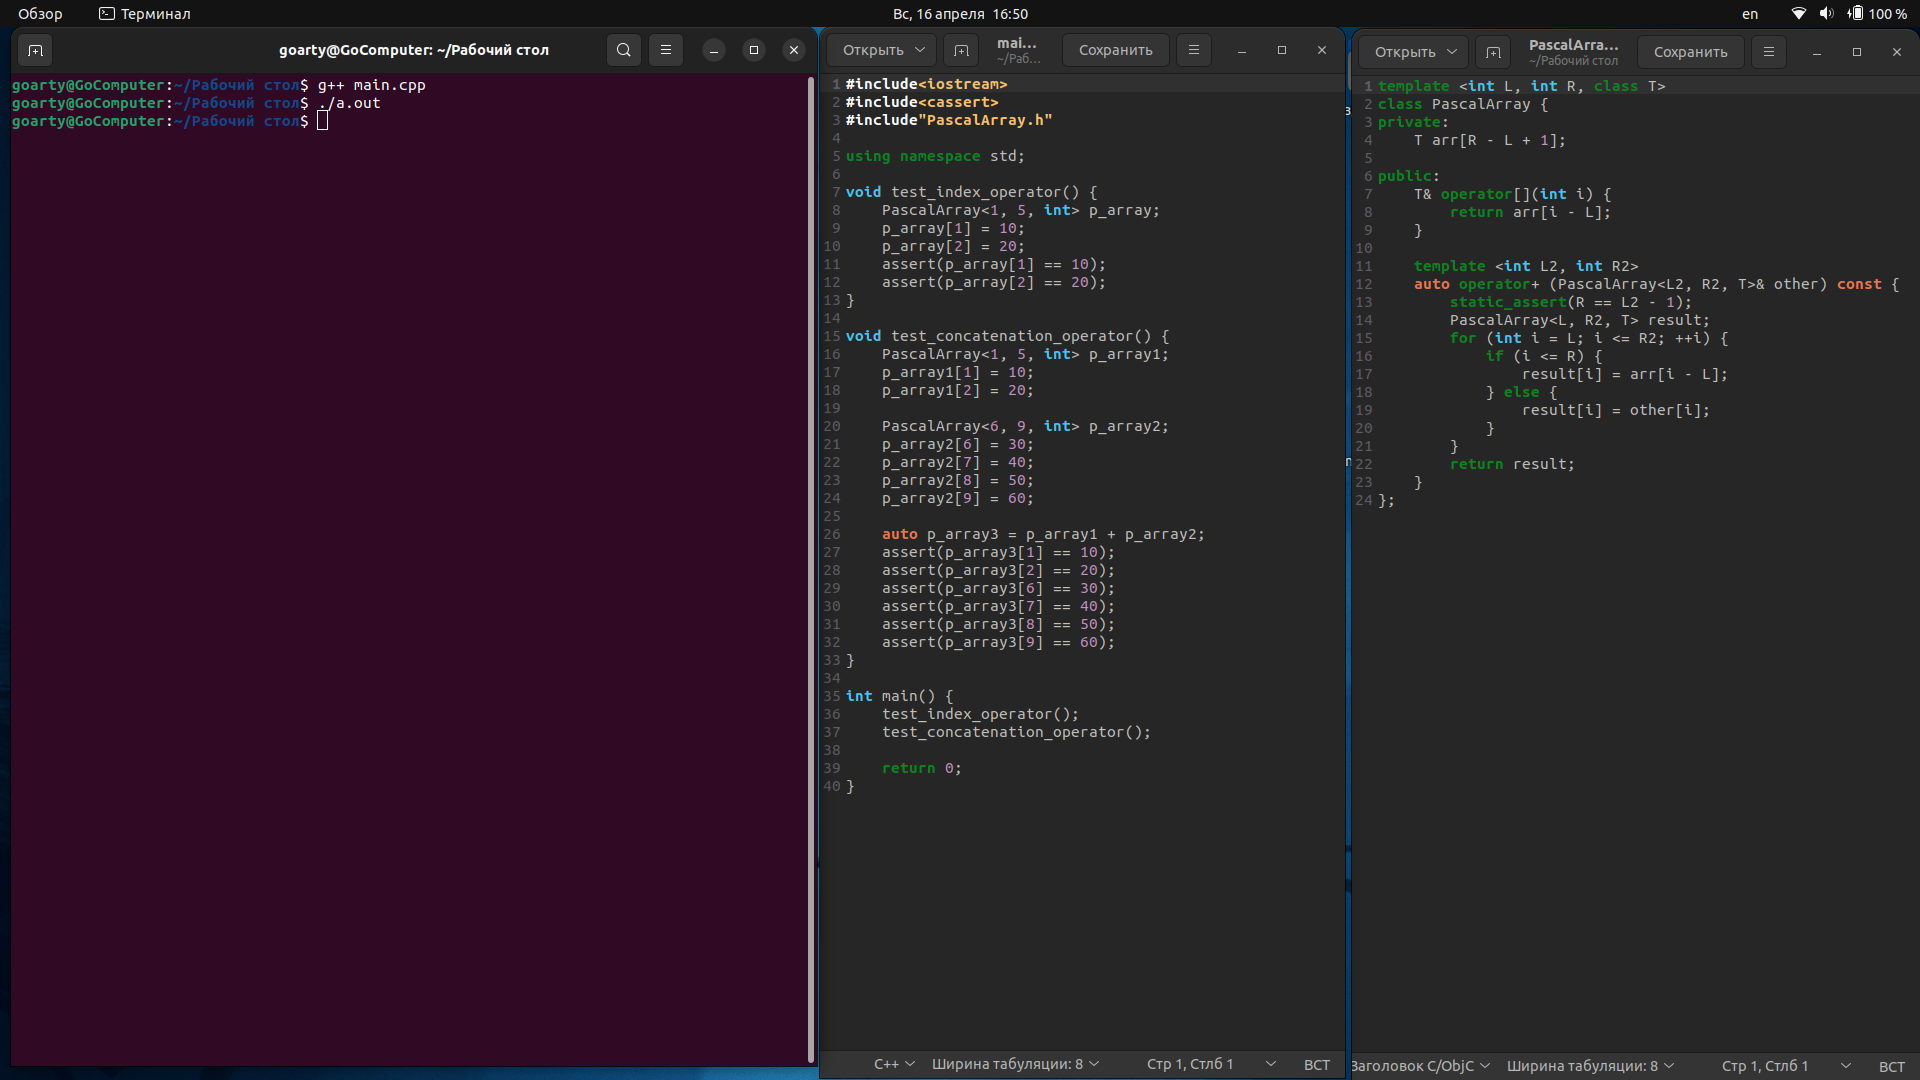
\includegraphics[width=0.8\textwidth]{picture_3.png}
\caption{Реализация 1.html}
\label{fig:picture_3.png}
\end{figure}

\begin{figure}[!htb]
	\centering
	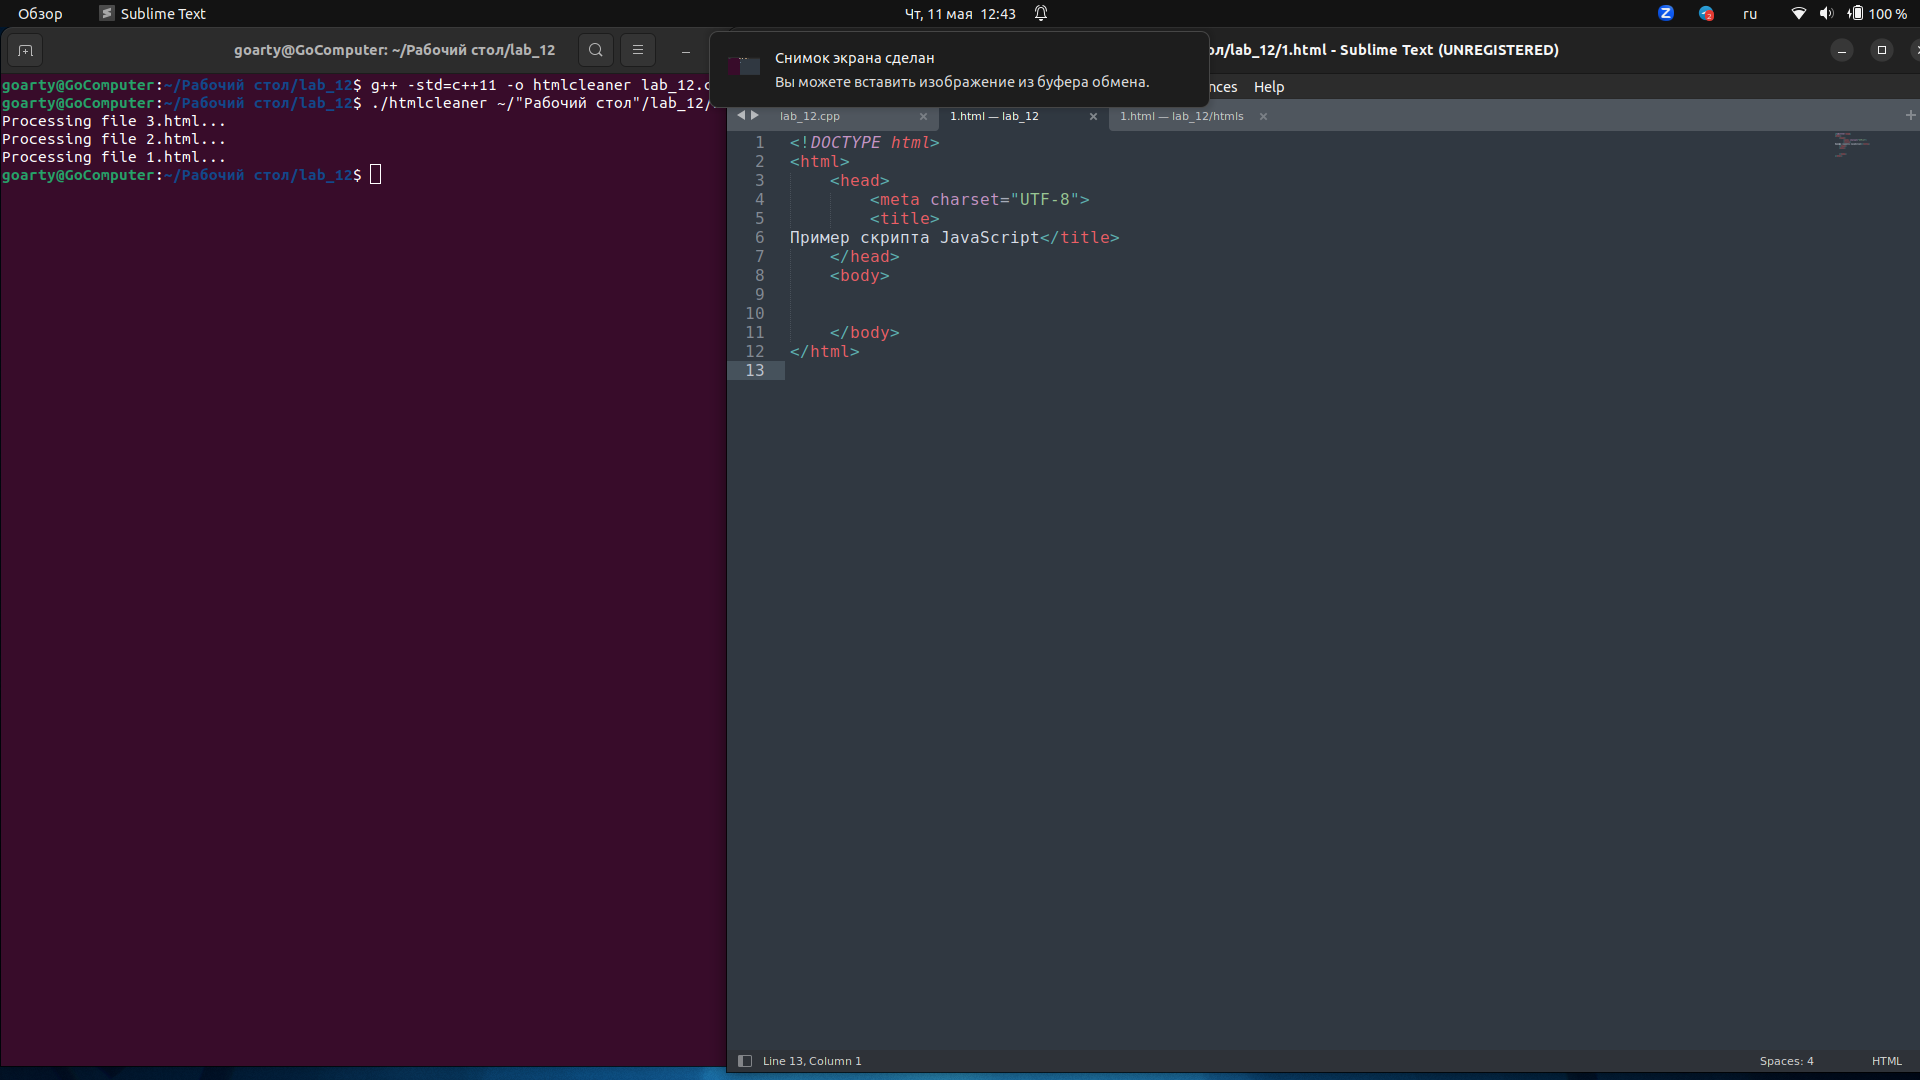
\includegraphics[width=0.8\textwidth]{picture_4.png}
\caption{Реализация 1.html(после работы програмы).java}
\label{fig:picture_4.png}
\end{figure}

\end{document}
